\documentclass{../../../oss-apphys}
\usepackage{bm}

\begin{document}
\genheader

\gentitle{1}{MOMENTUM, IMPULSE AND COLLISIONS}

\genmultidirections

\gengravity

\raggedcolumns
\begin{multicols}{2}

  \begin{enumerate}[leftmargin=18pt]

  \item A toy train car of mass \SI{3}{\kilo\gram} rolls to the left at
    \SI{2}{\metre\per\second} and collides with a \SI{4}{\kilo\gram} train
    car rolling to the right at \SI{1}{\metre\per\second}. The two cars stick
    together. The velocity of the cars after the collision is
    \begin{enumerate}[nosep,leftmargin=18pt,label=(\Alph*)]
    \item $2/7$ \si{\metre\per\second} to the left
    \item $2/7$ \si{\metre\per\second} to the right
    \item $4/7$ \si{\metre\per\second} to the left
    \item $4/7$ \si{\metre\per\second} to the right
    \item $9/7$ \si{\metre\per\second} to the right
    \end{enumerate}    
  \end{enumerate}
  
  \textbf{Questions \ref{impulse1}--\ref{impulse2}}. A force acts on a 2.0 kg
  mass during a time interval as shown in the graph.
  \begin{center}
    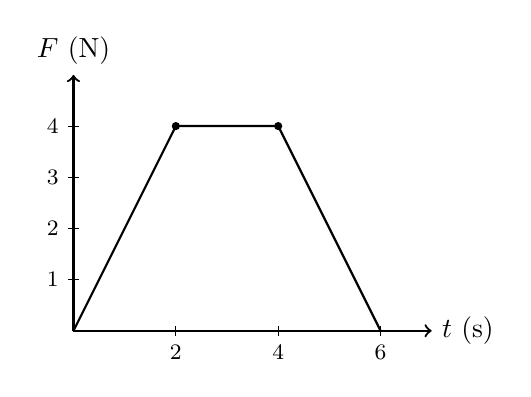
\begin{tikzpicture}[scale=.65]
      \draw[thick,->](0,0)--(7,0) node[pos=1,right]{$t$ (s)};
      \foreach \y in {1,...,4}{
        \draw(-.1,\y)--(.1,\y) node[pos=0,left]{\footnotesize\y};
      }
      \draw[thick,->](0,0)--(0,5) node[pos=1,above]{$F$ (N)};
      \foreach \x in {2,4,6}{
        \draw(\x,-.1)--(\x,.1) node[pos=0,below]{\footnotesize\x};
      }
      \draw[thick](0,0)--(2,4)--(4,4)--(6,0);
      \fill(2,4) circle(.08);
      \fill(4,4) circle(.08);
    \end{tikzpicture}
  \end{center}
  \begin{enumerate}[leftmargin=18pt,resume]
  \item The impulse given to the mass from $t=0$ to $t=\SI{6}{\second}$ is
    \label{impulse1}
    \begin{enumerate}[nosep,leftmargin=18pt,label=(\Alph*)]
    \item\SI{4 }{\newton\second}
    \item\SI{8 }{\newton\second}
    \item\SI{12}{\newton\second}
    \item\SI{16}{\newton\second}
    \item\SI{24}{\newton\second}
    \end{enumerate}
    
  \item If the initial speed of the mass is \SI{2}{\metre\per\second} at $t=0$,
    what is its speed at the end of 6 s?
    \label{impulse2}
    \begin{enumerate}[nosep,leftmargin=18pt,label=(\Alph*)]
    \item\SI{4}{\metre\per\second}
    \item\SI{6}{\metre\per\second}
    \item\SI{8}{\metre\per\second}
    \item\SI{10}{\metre\per\second}
    \item\SI{16}{\metre\per\second}
    \end{enumerate}
    \columnbreak
    
  \item Two steel balls, one of mass $m$ and the other of mass $2m$, collide and
    rebound in a perfectly elastic collision. Which of the following is
    conserved in this elastic collision?
    \begin{enumerate}[nosep,leftmargin=18pt,label=(\Alph*)]
    \item velocity only
    \item momentum only
    \item momentum and kinetic energy only
    \item momentum, velocity, and kinetic energy
    \item kinetic energy only
    \end{enumerate}
    \vspace{.8in}
    
  \item A rubber ball of mass $m$ strikes a wall with a speed $v$ at an angle
    $\theta$ below the normal line and rebounds from the wall at the same speed
    and angle above the normal line as shown. The magnitude of the change in
    momentum of the ball is
    \begin{center}
      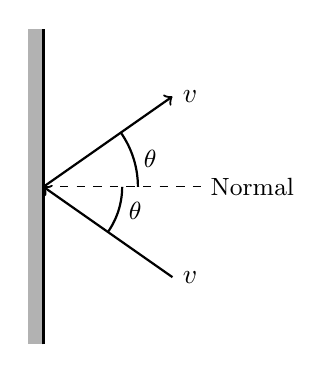
\begin{tikzpicture}
        \fill[gray!60](-.2,2) rectangle(0,-2);
        \draw[very thick](0,-2)--(0,2);
        \draw[dashed](0,0)--(2,0) node[right]{\small Normal};
        \draw[->,rotate=35, thick](0,0)--(2,0) node[right]{$v$};
        \draw[<-,rotate=-35,thick](0,0)--(2,0) node[right]{$v$};
        \draw[thick](1,0)  arc(0:-35:1)  node[midway,right]{\small$\theta$};
        \draw[thick](1.2,0)arc(0: 35:1.2)node[midway,right]{\small$\theta$};
      \end{tikzpicture}
    \end{center}
    \begin{enumerate}[nosep,leftmargin=18pt,label=(\Alph*)]
    \item $mv$
    \item $2mv$
    \item $mv\cos\theta$
    \item $2mv\cos\theta$
    \item  zero
    \end{enumerate}
    \columnbreak
    
  \item Two blocks are connected by a compressed spring and rest on a
    frictionless surface. The blocks are released from rest and pushed apart
    by the compressed spring. If one mass is twice the mass of the other,
    which of the following is the same for both blocks?
    \begin{enumerate}[nosep,leftmargin=18pt,label=(\Alph*)]
    \item magnitude of momentum
    \item acceleration
    \item speed
    \item kinetic energy
    \item potential energy
    \end{enumerate}
    
  \item A \SI{1000}{\kilo\gram} railroad car is rolling without friction on a
    horizontal track at a speed of \SI{3.}{\metre\per\second}. Sand is poured
    into the open top of the car for a time of \SI{5.}{\second}. The speed of
    the car after \SI{5.}{\second} is \SI{1.}{\metre\per\second}. The mass of
    the sand added to the car at the end of \SI{5.}{\second} is
    \begin{center}
      \pic{.23}{railroad-car-sand.png}
    \end{center}
    \begin{enumerate}[nosep,leftmargin=18pt,label=(\Alph*)]
    \item\SI{500 }{\kilo\gram}
    \item\SI{1000}{\kilo\gram}
    \item\SI{2000}{\kilo\gram}
    \item\SI{3000}{\kilo\gram}
    \item\SI{3500}{\kilo\gram}
    \end{enumerate}
    
  \item Two billiard balls are rolling to the right on a table as shown. The
    \SI{.4}{\kilo\gram} ball is moving faster than the \SI{.2}{\kilo\gram}
    ball, so it catches up and strikes it from behind at a slight angle.
    Immediately after the collision, the $y$-component of the
    \SI{.4}{\kilo\gram} ball is \SI{2}{\metre\per\second} downward.
    The $y$-component of the velocity of the \SI{.2}{\kilo\gram} ball must be
    \begin{center}
      \begin{tikzpicture}[scale=.5]
        \draw[dashed](-3,0)--(4,0) node[right]{\small$x$};
        \draw[dashed](0,-2)--(0,4) node[above]{\small$y$};
        \draw(.3,.3) circle(.3) node[above]{\small\;\;\;\SI{.2}{\kilo\gram}};
        \draw[->](.6,.3)--(1.6,.3) node[right]{\small$v_2$};
        \draw(-2.3,-.5) circle(.5) node[below left]{\small\SI{.4}{kg}\;\;};
        \draw[->](-1.8,-.5)--(-1,-.5) node[right]{\small$v_1$};
      \end{tikzpicture}
    \end{center}
    \begin{enumerate}[nosep,leftmargin=18pt,label=(\Alph*)]
    \item \SI{1}{\metre\per\second} upward
    \item \SI{2}{\metre\per\second} upward
    \item \SI{1}{\metre\per\second} downward
    \item \SI{2}{\metre\per\second} downward
    \item \SI{4}{\metre\per\second} upward
    \end{enumerate}

    
  \item A \SI{.3}{\kilo\gram} baseball at rest on a tee is struck by a bat. The
    ball leaves the at with a speed of \SI{20}{\metre\per\second} at an angle
    of \ang{45} above the horizontal. The magnitude of the impulse imparted to
    the baseball by the bat is most nearly
    \begin{enumerate}[nosep,leftmargin=18pt,label=(\Alph*)]
    \item\SI{2}{\newton\second}
    \item\SI{6}{\newton\second}
    \item\SI{12}{\newton\second}
    \item\SI{16}{\newton\second}
    \item\SI{20}{\newton\second}
    \end{enumerate}
    
  \item Two ice skaters, a large man and a small woman, are initially at rest
    and holding each other's hands. They push away horizontally. Afterward,
    which of the following statements is true?
    \begin{enumerate}[nosep,leftmargin=18pt,label=(\Alph*)]
    \item They have equal and opposite kinetic energies.
    \item The have equal and opposite momenta.
    \item The large man applies a greater force to the small woman.
    \item The small woman applies a greater force to the large man.
    \item They recoil with equal and opposite velocities.
    \end{enumerate}
    \vspace{.8in}
    
  \item A known net force $F$ acts on an unknown mass for a known time
    $\Delta t$. From this information, you could determine the
    \begin{enumerate}[nosep,leftmargin=18pt,label=(\Alph*)]
    \item change in kinetic energy of the object
    \item change in velocity of the object
    \item acceleration of the object
    \item mass of the object
    \item change in momentum of the object
    \end{enumerate}
    \vspace{.8in}
    
  \item A \SI{100}{\kilo\gram} cannon sits at rest with a \SI{1}{\kilo\gram}
    cannonball in the barrel. The cannonball is fired with a speed of
    \SI{50}{\metre\per\second} to the right, causing the cannon to recoil with
    a speed of \SI{.5}{\metre\per\second} to the left. The velocity of the
    center of mass of the cannon-cannonball system is
    \begin{enumerate}[nosep,leftmargin=18pt,label=(\Alph*)]
    \item zero
    \item\SI{5}{\metre\per\second} to the right
    \item\SI{5}{\metre\per\second} to the left
    \item\SI{50}{\metre\per\second} to the right
    \item\SI{50}{\metre\per\second} to the left
    \end{enumerate}
  \end{enumerate}
  \columnbreak

  \textbf{Questions \ref{explode1}--\ref{explode2}}. An object has a mass $4m$.
  The object explodes into three pieces of mass $m$, $m$, and $2m$. The two
  pieces of mass $m$ move off at right angles to each other with the same
  momentum $mv$, as shown.
  \begin{center}
    \begin{tikzpicture}[scale=.6]
      \draw[thick,dashed](-1.5,0)--(3,0);
      \draw[thick,dashed](0,-1.5)--(0,3);
      \draw[thick](0,0) circle(.5);
      \fill[thick](-1.5,0) circle(.15) node[above]{\small $m$};
      \fill[thick](0,-1.5) circle(.15) node[right]{\small $m$};
      \draw[very thick,->](-1.5,0)--(-3,0)node[left]{\small$mv$};
      \draw[very thick,->](0,-1.5)--(0,-3)node[below]{\small$mv$};
    \end{tikzpicture}
  \end{center}
  
  \begin{enumerate}[leftmargin=18pt,resume]
  \item The speed of mass $2m$ after the explosion is
    \label{explode1}
    \begin{enumerate}[nosep,leftmargin=18pt,label=(\Alph*)]
    \item $2v$
    \item $\displaystyle\sqrt2v$
    \item $\displaystyle\frac{\sqrt2}2v$
    \item $\displaystyle\frac{\sqrt2}3v$
    \item $\displaystyle\frac{\sqrt3}2v$
    \end{enumerate}
    
  \item The direction of velocity of mass $2m$ is
    \label{explode2}
    \begin{enumerate}[nosep,leftmargin=18pt,label=(\Alph*)]
    \item $\rightarrow$
    \item $\swarrow$
    \item $\downarrow$
    \item $\nearrow$
    \item $\uparrow$
    \end{enumerate}
  
  \item A block of mass $m$ is moving to the right with a speed $v_0$ on a
    horizontal surface of negligible friction when it explodes. The explosion
    causes the block to break into two pieces, each of which moves in the
    horizontal direction. One piece of mass $m/4$ moves to the left with a
    speed of $2v_0$. What is the velocity of the other piece?
    \begin{enumerate}[nosep,leftmargin=18pt,label=(\Alph*)]
    \item$2v_0$ to the right
    \item$v_0$ to the right
    \item$3⁄4 v_0$ to the right
    \item$1⁄2 v_0$ to the right
    \item$1⁄4 v_0$ to the left
    \end{enumerate}
  \end{enumerate}
  \columnbreak
  
  \textbf{Questions \ref{3masses1}--\ref{3masses2}}. Three identical masses can
  slide freely on a horizontal surface as shown. The first mass moves with a
  speed of \SI{3.}{\metre\per\second} toward the second and third masses, which
  are initially at rest. The first and second mass collide elastically, and
  then the second and third masses collide inelastically.
  \begin{center}
    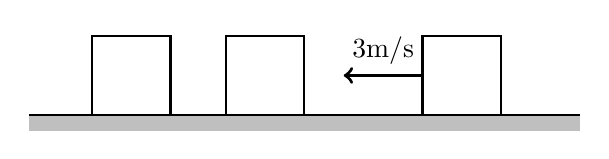
\begin{tikzpicture}
      \fill[gray!50](0,0) rectangle(7,-.2);
      \draw[thick](0,0)--(7,0);
      \draw[thick](.8,0) rectangle(1.8,1);
      \draw[thick](2.5,0) rectangle(3.5,1);
      \draw[thick](5,0) rectangle(6,1);
      \draw[very thick,->](5,.5)--(4,.5) node[midway,above]{\SI{3}{m/s}};
    \end{tikzpicture}
  \end{center}
  \begin{enumerate}[leftmargin=18pt,resume]
  \item The speed of the second mass after the collision is
    \label{3masses1}
    \begin{enumerate}[nosep,leftmargin=18pt,label=(\Alph*)]
    \item zero
    \item\SI{1.5}{\metre\per\second}
    \item\SI{3.}{\metre\per\second}
    \item\SI{6.}{\metre\per\second}
    \item\SI{9.}{\metre\per\second}
    \end{enumerate}

  \item The speed of the second and third masses after they collide
    inelastically is
    \label{3masses2}
    \begin{enumerate}[nosep,leftmargin=18pt,label=(\Alph*)]
    \item zero
    \item\SI{1.5}{\metre\per\second}
    \item\SI{3.0}{\metre\per\second}
    \item\SI{6.0}{\metre\per\second}
    \item\SI{9.0}{\metre\per\second}
    \end{enumerate}
  \end{enumerate}

  \textbf{Questions \ref{boy1}--\ref{boy2}}. A \SI{20}{\kilo\gram} boy runs at
  a speed of \SI{3}{\metre\per\second} and jumps onto a \SI{40}{\kilo\gram}
  sled on frictionless ice that is initially at rest. The boy and the sled then
  move together for a short time.

  \begin{enumerate}[resume,leftmargin=18pt]
  \item The speed of the boy and sled after he jumps on it is
    \label{boy1}
    \begin{enumerate}[nosep,leftmargin=18pt,label=(\Alph*)]
    \item\SI{0.5}{\metre\per\second}
    \item\SI{0.8}{\metre\per\second}
    \item\SI{1.0}{\metre\per\second}
    \item\SI{1.5}{\metre\per\second}
    \item\SI{2.0}{\metre\per\second}
    \end{enumerate}
    
  \item While the boy and sled are moving, he jumps off the back of the sled in
    such a way the boy is at rest, and the sled continues to move forward.
    The speed of the sled after the boy jumps off is
    \label{boy2}
    \begin{enumerate}[nosep,leftmargin=18pt,label=(\Alph*)]
    \item\SI{1.5}{\metre\per\second}
    \item\SI{2.0}{\metre\per\second}
    \item\SI{3.0}{\metre\per\second}
    \item\SI{4.5}{\metre\per\second}
    \item\SI{6.0}{\metre\per\second}
    \end{enumerate}
    \columnbreak
    
  \item A 1.0 kg block is released from rest from a height $h$ at the top of a
    fixed curved ramp of negligible friction. The block slides down the
    ramp and collides with another block of mass 1.5 kg at rest at the
    bottom of the ramp. The two blocks stick together and move with a
    speed of \SI{5}{\metre\per\second}. The height $h$ from which the 1.0 kg
    block began is
    \begin{enumerate}[nosep,leftmargin=18pt,label=(\Alph*)]
    \item 0.8 m
    \item 1.2 m
    \item 1.8 m
    \item 2.8 m
    \item 7.8 m
    \end{enumerate}

  \item A dart of mass $m$ is fired into a wooden block of mass $4m$ that hangs
    from a string. The dart and block then rise to a maximum height $h$. An
    expression for the initial speed $v_0$ of the dart before striking the block
    is
    \begin{enumerate}[nosep,leftmargin=18pt,label=(\Alph*)]
    \item$\sqrt{gh}$
    \item$\sqrt{2gh}$
    \item$\sqrt{50gh}$
    \item$\sqrt{100gh}$
    \item$\sqrt{250gh}$
    \end{enumerate}

  \item A mass $m_1$ initially moving at speed $v_0$ collides with and sticks
    to a spring attached to a second, initially stationary mass $m_2$. The two
    masses continue to move to the right on a frictionless surface as the
    length of the spring oscillates. At the instant that the spring is
    maximally extended, the velocity of the first mass is
    \begin{center}
      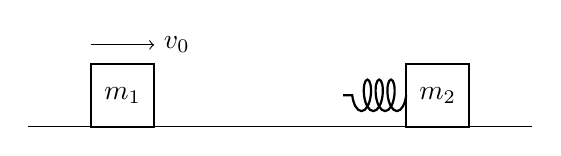
\begin{tikzpicture}[scale=.8]
        \draw[->](1,1.3)--(2,1.3) node[pos=1,right]{$v_0$};
        \draw(0,0)--(8,0);
        \draw[thick](1,0) rectangle (2,1) node[midway]{$m_1$};
        \draw[thick](6,0) rectangle (7,1) node[midway]{$m_2$};
        \draw[thick,
          decoration={aspect=.4,segment length=1.5mm, amplitude=2mm,coil},
          decorate] (6,.5)--(5,.5);
      \end{tikzpicture}
    \end{center}
    \begin{enumerate}[nosep,leftmargin=18pt,label=(\Alph*)]
    \item $v_0$
    \item $m_1^2v_0/(m_1+m_2)^2$
    \item $m_2v_0/m_1$
    \item $m_1v_0/m_2$
    \item $m_1v_0/(m_1+m_2)$
    \end{enumerate}
  \end{enumerate}
  \columnbreak
  
  \textbf{Questions \ref{ramps1}--\ref{ramps2}}. A small block of mass $m$
  slides on a horizontal frictionless surface toward a ramp of mass $3m$ which
  is also free to move on the surface. The small block slides up to a height
  $h$ on the ramp with no friction (Figure I), then they move together (Figure
  II), and the small block slides back down the ramp to the horizontal surface
  (Figure III). Both the block and the ramp continue to slide on the horizontal
  surface after they separate.
  \begin{center}
    \pic{.3}{Figs123.png}
  \end{center}
  \begin{enumerate}[resume,leftmargin=18pt]  
  \item Which of the following is true regarding the conservation laws
    throughout this process?
    \label{ramps1}
    \begin{enumerate}[nosep,leftmargin=18pt,label=(\Alph*)]
    \item Kinetic energy is conserved from Figure I to Figure II.
    \item Momentum is conserved from Figure I to Figure III.
    \item Kinetic energy is conserved from Figure II to Figure III.
    \item Potential energy is conserved from Figure I to Figure II.
    \item Potential energy is conserved from Figure II to Figure III.
    \end{enumerate}
    \vspace{.8in}
    
  \item Which of the following is a true statement regarding Figure III?
    \label{ramps2}
    \begin{enumerate}[nosep,leftmargin=18pt,label=(\Alph*)]
    \item The small block is moving to the left and the ramp is moving to the
      right.
    \item The small block is moving to the right and the ramp is moving to the
      left.
    \item The small block is moving to the right and the ramp is moving to the
      right.
    \item The small block is moving to the left and the ramp is moving to the
      left.
    \item The small block and the large block are moving with the same velocity.
    \end{enumerate}    
    \columnbreak
    
  \item Two masses moving along the coordinates axes as shown collide at the
    origin and stick to each other. What is the angle $\theta$ that the final
    velocity that makes with the $x$-axis?
    \begin{center}
      \begin{tikzpicture}[scale=.7]
        \draw(-4,0)--(4,0);
        \draw(0,-3)--(0,3);
        \draw[very thick,->](-3,0)--(-1,0)node[midway,below]{\small$\mb{v}_1$};
        \draw[very thick,->](0,-2)--(0,-1) node[midway,right]{\small$\mb{v}_2$};
        \draw[very thick,->](0,0)--(1.3,1.3)node[pos=1,right]{\small$\mb{v}_f$};
        \draw[fill=gray](-3,0) circle(.2) node[above]{\small$m_1$};
        \draw[fill=gray](0,-2) circle(.2) node[right]{\small$m_2$};
        \draw[<->] (.75,0) arc(0:45:.75) node[pos=.6,right]{\small$\theta$};
      \end{tikzpicture}
    \end{center}
    \begin{enumerate}[nosep,leftmargin=18pt,label=(\Alph*)]
    \item $\tan^{-1}(v_2/v_1)$
    \item $\tan^{-1}[m_1v_1/(m_1+m_2)]$
    \item $\tan^{-1}(m_1v_2/m_2v_1)$
    \item $\tan^{-1}(m_2v_2^2/m_1v_1^1)$
    \item $\tan^{-1}(m_2v_2/m_1v_1)$
    \end{enumerate}
    \columnbreak
    
  \item A mass traveling in the $+x$ direction collides with a mass at rest.
    Which of the following statements is true?
    \begin{enumerate}[nosep,leftmargin=18pt,label=(\Alph*)]
    \item After the collision, the two masses will move with parallel velocities
    \item After the collision, the masses will move with anti-parallel
      velocities
    \item After the collision, the masses will both move along the $x$-axis
    \item After the collision, the $y$-components of the velocities of the two
      particles will sum to zero.
    \item None of the above
    \end{enumerate}
  \end{enumerate}
\end{multicols}
\newpage


\genfreetitle{1}{MOMENTUM, IMPULSE, COLLISIONS, AND CENTER OF MASS}{4}

\genfreedirections

\begin{enumerate}[leftmargin=15pt]
  
  % TAKEN FROM THE 2016 AP PHYSICS 1 EXAM FREE-RESPONSE QUESTION #2
\item (Suggested time 25 minutes) A new kind of toy ball is advertised to
  ``bounce perfectly elastically'' off hard surfaces. A student suspects,
  however, that no collision can be perfectly elastic. The student hypothesizes
  that the collisions are very close to being perfectly elastic for low-speed
  collisions but that they deviate more and more from being perfectly elastic
  as the collision speed increases.
  \begin{enumerate}[leftmargin=18pt,noitemsep]
  \item Design an experiment to test the student's hypothesis about collisions
    of the ball with a hard surface. The student has equipment that would
    usually be found in a school physics laboratory.
    \begin{enumerate}[leftmargin=18pt,noitemsep]
    \item What quantities would be measured?
    \item What equipment would be used for the measurements, and how would that
      equipment be used?
    \item Describe the procedure to be used to test the student's hypothesis.
      Give enough detail so that another student could replicate the experiment.
    \end{enumerate}
  \item Describe how you would represent the data in a graph or table. Explain
    how that representation would be used to determine whether the data are
    consistent with the student's hypothesis.
  \item A student carries out the experiment and analysis described in parts
    (a) and (b). The student immediately concludes that something went wrong in
    the experiment because the graph or table shows behavior that is elastic
    for low-speed collisions but appears to violate a basic physics principle
    for high-speed collisions.
    \begin{enumerate}[leftmargin=18pt,noitemsep]
    \item Give an example of a graph or table that indicates nearly elastic
      behavior for low-speed collisions but appears to violate a basic physics
      principle for high-speed collisions.
    \item State one physics principle that appears to be violated in the graph
      or table given in part (c)i. Several physics principles might appear to
      be violated, but you only need to identify one.

    \item Briefly explain what aspect of the graph or table indicates that th
      e physics principle is violated, and why.
    \end{enumerate}
  \end{enumerate}
  \newpage
  
\item The Ballistic Pendulum. To determine the muzzle speed of a gun, a bullet
  is shot into a mass $M$ from a string as shown below, causing $M$ to swing
  upward through a maximum angle of $\theta$.
  \begin{center}
    \pic{.4}{ballastic.png}
  \end{center}
  \begin{enumerate}[noitemsep]
  \item What is the speed of $M$ the instant after the bullet lodges in it?
    \vspace{1.25in}
  \item What is the speed of the bullet before it hits $M$?
    \vspace{1.25in}
  \item What is the tension in the string at the highest point of the pendulum's
    swing (when the string makes an angle of $\theta$ with the vertical as
    shown)?
  \end{enumerate}
  \newpage
  
\item An 800.0-kg car is traveling along a wet road at a velocity of
  \SI{25.5}{\metre\per\second}. A \num{1000.}-kg car is traveling along the
  same road in the same direction at \SI{34.7}{\metre\per\second}. The two cars
  collide and lock together. Answer the following questions.
  \begin{enumerate}[leftmargin=18pt]
  \item The two interlocked cars proceed at what velocity after the collision?
  \item Compare the kinetic energy of the two-car system immediately before
    the collision and after the collision.
  \item Discuss any transfer of energy that occurs, and explain whether this is
    an elastic or inelastic collision.
  \item If the coefficient of sliding friction between the tires of the cars
    and the wet pavement is 0.7, calculate the force of friction.
  \item  How long does it take for the two interlocked cars to come to a
    complete stop on the wet pavement?
  \end{enumerate}
  \newpage
  
\item A stream of glass beads, each with a mass of 0.5 g, comes out of a
  horizontal tube at 100 per second. The beads fall a distance of 0.5 m to a
  balance pan and bounce back to their original height as shown in the figure
  below. How much mass must be placed in the other pan of the balance to keep
  the pointer at zero?
  \begin{center}
    \pic{.5}{balance.jpg}
  \end{center}
  \vspace{\stretch{1}}
\end{enumerate}
\end{document}
